\scanpage{69}
\figure{\begin{tikzpicture}
\node[rotate=180,inner sep=0pt]{\begin{minipage}{14cm}\small
\begin{tabular}{l@{\hspace{.8cm}}l}
UNIVERSITÉ DES SCIENCES&\\
ET TECHNIQUES DU LANGUEDOC&ACADÉMIE DE MONTPELLIER\\
MONTPELLIER II&\\
Place Eugène Bataillon&\\
34060 MONTPELLIER CEDEX&
\end{tabular}

Tél. : 63.91.44 -- Télex : USTMONT 49944 F

\begin{tabular}{l@{\hspace{3cm}}l}
FA/RR&Montpellier, le\quad\unsure{16|06} FEVR. 1979\quad19
\end{tabular}

01011
\begin{flushright}
Le PRESIDENT de l'UNIVERSITE\\
à\hspace*{5cm}\\
Monsieur le Professeur MICALI\\
Directeur de l'U.E.R. 5
\end{flushright}
\vspace{1cm}
Monsieur le Directeur et Cher Collègue,

\hspace*{1.2cm}Le Bureau du Conseil scientifique dans sa réunion du 8 Février 1979 a réexaminé votre demande de subvention pour l'a-\\ménagement de la bibliothèque de mathématiques.

\hspace*{1.2cm}Il semble difficile d'accorder des crédits sur le bud-\\get ``recherche'' pour couvrir des frais d'aménagement de locaux. En conséquence, il a été envisagé de vous accorder une avance de 50.000 F. Pour vous permettre de rembourser cette somme, le bureau étudiera la possibilité de revaloriser les ``points chercheurs'' at-\\tribués aux mathématiciens.

\hspace*{1.2cm}Je vous signale toutefois que cette avance ne pourra être mise à votre disposition que dans la mesure où la procédure compta-\\ble à utiliser aura été définie et qu'elle vous aura été notifiée.

\hspace*{1.2cm}Veuillez agréer, Monsieur le Directeur et Cher Collègue, l'expression de mes sentiments les meilleurs.

\begin{flushright}
Le Président :\\[4pt]
\begin{tikzpicture}[scale=.6]
\node[font=\itshape]at(0,0){\unsure{L. Thaler}};
\draw(-1.7,.25)to[bend right=65](-1.43,-.23);\draw(-.8,.38)to[bend right=35](-.4,.35)--(-.5,-.32);\draw(-.1,.21)to[bend right=60](.3,-.18)to[bend right=30](.6,.14)to[bend right=45](1,-.18)to[bend right=20](1.6,-.2);
\end{tikzpicture}\\
L. THALER\\[3pt]
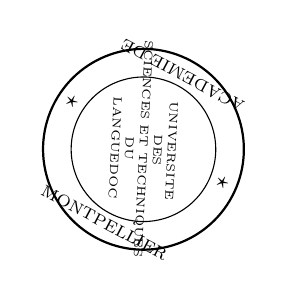
\begin{tikzpicture}[scale=.85,rotate=-28,transform shape]
\draw[thick](0,0)circle(1.5);\draw(0,0)circle(1.08);
\node[font=\scriptsize,rotate=180]at(0,1.25){\unsure{ACADEMIE DE}};
\node[font=\scriptsize]at(0,-1.24){MONTPELLIER};\node at(-1.28,.13){$\star$};\node at(1.27,.12){$\star$};
\node[font=\tiny,align=center,rotate=-65]at(0,0){UNIVERSITE\\\unsure{DES}\\SCIENCES \unsure{ET TEC}HNIQUES\\DU\\LANGUEDOC};
\end{tikzpicture}
\end{flushright}
\end{minipage}};
\end{tikzpicture}}
\mspage{68}
